\chapter{Design \& Implementation}
\label{ch:design-implementation}

\section{Language \& Libraries}

% \begin{itemize}
%     \item Python as pre-existing machine learning frameworks
%     \item Tensorflow vs PyTorch (Tensorflow seemed nicer and more base code, first code seen for proof of concept was in tensorflow)
%     \item mutually exclusive due to CUDA implementations
% \end{itemize}

\subsection{Python}

When choosing a language to code this project in Python\footnote{\url{https://www.python.org}} was a clear choice. Whilst other languages offer better speed (C++\footnote{\url{https://cplusplus.com/}}, Rust\footnote{\url{https://www.rust-lang.org/}}), Python's advantage comes from its libraries.

Libraries are modular pieces of code written by other developers that can be integrated into a new software to make common tasks easier. In Python this is accomplished using the \verb|import| and \verb|from| syntax. Libraries vastly simplify coding as they can vastly reduce complex problems to simple functions. This is especially useful when dealing with complex machine learning functions, advanced mathematical algorithms such as Adam can be reduced to an import. Many Python libraries are written in lower-level languages like C or C++, allowing Python code to benefit from high performance while maintaining ease of use.

The vast majority of popular packages have a Python implementation that can be easily installed by the Python Package Index\footnote{\url{https://pypi.org/}}. Especially for machine learning, Python has some of the largest collection of relevant libraries of any language and is therefore the language of choice for this project.

\subsection{PyTorch versus TensorFlow}

There are many machine learning frameworks in Python, however the primary two are PyTorch\cite{paszke2019pytorch} and TensorFlow\cite{abadi2016tensorflow}. They both offer near identical feature sets and performance so choosing between them is not a simple matter.

PyTorch was created by Meta in 2019. It is a lot newer and viewed as a more ``pythonic" framework\cite{chirodea2021comparison}. To be more ``pythonic" is to be more developer-friendlier by providing a simple interface to the library that developers already familiar with Python should easily pick up on. PyTorch supports a dynamic computation graph which enables for dynamic changes of model architectures.

TensorFlow is a much more mature framework by Google releasing in 2015. It offers similar abstractions as PyTorch but is widely viewed to be slightly harder to develop in\cite{chirodea2021comparison}. TensorFlow uses an eager computation graph meaning no changes to model architectures can be made once a model is defined. Whilst this reduces flexibility during runtime, it allows for more optimisations to be made to the model architecture meaning greater accuracy, smaller model architectures, and sometimes quicker computations. TensorFlow also scales effectively running as efficiently as possible on desktop computers to large GPU clusters.

Unfortunately, TensorFlow and PyTorch are mutually exclusive. Both rely on separate versions of the CUDA backend to allow for GPU acceleration on NVIDIA architectures. Whilst this can be accomplished using virtually environments and other work arounds it is generally recommended to use one or the other.

Due to their similarities, there is no clear choice between PyTorch and TensorFlow. Some trends have emerged, however, with PyTorch being used for research and development work where iterative improvements are desired whereas as TensorFlow is employed for production environments. 

TensorFlow was chosen for this project for a number of reasons. Firstly, the flexibility that PyTorch offers is less important to this project as all models being used have had their architectures pre-defined. On the other hand, TensorFlow's ability to scale and optimise for the compute resources will be valuable for this project as it will be developed on smaller desktops but the final evaluation loops will be run on large GPU clusters. Furthermore, after trying out both TensorFlow and PyTorch, the author preferred the overall syntax of TensorFlow.

\section{Proof of Concept}
\label{sec:concept-design}

% \begin{itemize}
%     \item Re-use oriented design
%     \item Quick and dirty
%     \item test my theory
%     \item explain methodologies
% \end{itemize}

To validate whether blink-based DeepFake detection is resistant to adversarial noise, it was decided to construct a proof of concept during the Christmas holiday. As it is intended to be a small test-bed, small flaws in the design are acceptable. Therefore, it makes sense to use pre-existing models, solutions, and implementations where possible in order to speed up development.

The overall architecture of blink-based DeepFake detection is relatively simple. First, the landmarks around the face are computed to determine for every frame to generate an EAR-time graph. The graph can then be analysed to determine whether the video is real or not. 

\begin{algorithm}
    \caption{Overall architecture of a blink-based DeepFake detector}
    \label{alg:blink-based}
    \begin{algorithmic}
        \State{ears $\gets$ \{\}}
        \For{frame $\in$ video}
            \State landmarks $\gets$ \textsc{GetLandmarks}(frame)
            \State ear $\gets$ \textsc{CalculateEAR}(landmarks)
            \State \textsc{Append}(ears, ear)
        \EndFor
        \State classification $\gets$ \textsc{EARAnalysis}(ears)
    \end{algorithmic}
\end{algorithm}

It was decided to use an EAR-based approach over a custom blink model, because it allows for complex analysis. EAR data is more precise than the binary open/close of a custom model, allowing for analysis of not just frequency of blinks but more subtle details like how the blink starts and ends, the velocity of the eye, and whether the eye consistently returns to the same position when open. The flaws in EAR noted by Ictu Oculi\cite{li2018ictu} are valid but they rely on the eye landmarks being unreliably marked, with sufficiently advanced models trained with occlusions this can be overcome. 

To calculate the EAR, the six landmarks around the eye need to be located. Google's MediaPipe\cite{lugaresi2019mediapipe} was used for this purpose. It is designed to run in real-time on mobile devices and other edge compute resources and hence is very light weight and fast. MediaPipe produces 478 landmarks in three dimensions that cover the entire face, a subset of twelve (six landmarks per eye) is then used to be the six landmarks for EAR. From the six landmarks, the EAR can be calculated using Equation \ref{eq:ear} and the average taken for the final EAR-time graph. 

EAR analysis is performed using the hybrid of DeepVision\cite{jung2020deepvision} and Ictu Oculi\cite{li2018ictu} by counting the number of blinks in the EAR graph and comparing that to the human average. DeepVision's database was viewed as too time-consuming to produce and the simplicity of Ictu Oculi's approach was appealing for its speed advantage. In experiments, DeepVision's threshold of two standard deviations below the mean proved to be to inconsistent so a revised threshold of half a standard deviation above the minimum EAR value was chosen. The average human blinks 14 times per minute\cite{schiffman1990sensation}, DeepFakes will blink less than this and so if the subject of the video blinks less than 14 times a minute, the video is deemed as a fake.

For traditional detectors, both ResNet and VGG architectures have been proven vulnerable to adversarial noise\cite{gandhi2020adversarial}. A ResNet-based DeepFake detector was implemented using an implementation from Tiwari\cite{tiwari2024deepfake}, a VGG-detector was implemented using a header from Krishna et al\cite{krishna2022deepfake} but the backbone was upgraded to VGG19 following research from Yadav et al\cite{yadav2024deepfake}. To extend frame-by-frame detection to entire videos, each frame in a video is analysed independently. If the frame is classified as fake then a counter is incremented by one. If the counter exceeds a given threshold (set as one hundred frames), the video is classed as fake.

Adversarial noise was added to images using the Foolbox library\cite{rauber2017foolbox}\cite{rauber2017foolboxnative}. FGSM was used as the method for noise due to its known effectiveness and speed\cite{gandhi2020adversarial}. $\epsilon$ was set to 0.1. To replicate real life scenarios, noise was only added to faked videos and all models were solely trained on original videos, not noisy ones.

The models were trained on a subset of fifty real and fifty fake videos from the FaceForensics++ dataset\cite{roessler2018faceforensics}. Testing was run over a further fifty real and fifty fake videos. The results of the tests can be found in Section \ref{sec:concept-results}. FaceForensics++ was chosen as it was the most robust dataset available at the time. More have been tested in the main code. Hyperparameters for the VGG and ResNet models were left the same as the original implementations. To reduce overfitting, only one frame per second was extracted and used for training.

\section{Main DeepFake Detection Algorithm}

% \begin{itemize}
%     \item pseudocode of main algorithm
%     \item if at any point something fails, mark as fake (ensures resiliency)
%     \item emphasise each part is interchangeable
% \end{itemize}

The main DeepFake detection algorithm is similar to the one discussed in the proof of concept (Algorithm \ref{alg:blink-based}) in terms of structure. The code in the main algorithm is an alteration of the subroutine calls, making each subroutine return more accurate results. Other improvements were made such as general improving speed and modularity of the code. To further improve testing and evaluation, a number of different options for each component were developed as each section of the algorithm is interchangeable. 

To improve resiliency against adversarial noise attacks, the entire algorithm is fail negative. If any section of the algorithm were to fail then the video would be deemed a fake. For example, if no facial landmarks are detected in a frame, then the video is declared fake.

\subsection{Eye Landmark Detection}

% \begin{itemize}
%     \item EAR needs 6 points per eye so lets get them
%     \item Facial landmarking is a common superset problem
%     \item Introduce 68 landmarks and datasets
%     \item Most popular ones aren't viable as built to be small to fit in a package (dlib, opencv...) or to run on a phone (mediapipe)
% \end{itemize}

To determine the EAR in a specific frame, the six landmarks around each eye need to be located. There are a large number of Python packages which come with facial landmarking features, unfortunately most of these are unsuitable for use in a state of the art detector as they are insufficiently accurate. The models included in packages are either compressed for ease of distribution or optimised to run on devices with reduced computational capabilities. 

\subsubsection{Face cropping}

One common feature across all facial landmarking models is that they perform best when the face being landmarked fills the entire frame. As such, it is incredibly useful to have a preprocessing step which crops a frame to just the faces in the frame using a face detector model. 

One of the most efficient models available is YuNet\cite{wu2023yunet}. YuNet is designed to run in real time (approximately 1 millisecond per frame) on a CPU, whilst retaining a high degree of accuracy. It only contains 75,856 parameters, with many models requiring fifty times more parameters to reach similar levels of accuracy. More parameters means longer computation times, which was deemed unacceptable for a model designed to run on edge devices. With neural networks, quicker computation times often come at the expense of reduced accuracy; whilst this is still the case with YuNet, it still achieves ``similar accuracy to other small models" on standardised benchmarks. OpenCV contains an implementation of YuNet for use in Python\cite{yunetpyton}.

A more accurate CNN for detecting faces is Multitask Cascaded Convolutional Networks (MTCNN)\cite{zhang2016joint}. MTCNN is more accurate, achieving 0.851 mean average precision on benchmarks, compared to YuNet's 0.836. The accuracy comes with a significant speed decrease. Where YuNet takes one millisecond per frame, MTCNN takes ten milliseconds. The MTCNN library\cite{centeno2024mtcnn} is a popular Python implementation of MTCNN.

To attain the optimal combination of speed and accuracy both YuNet and MTCNN are used to identify faces in a video. An initial pass on all frames is done via YuNet, if no faces are found in a frame then MTCNN is used to identify the faces. To improve the performance of MTCNN, faces are processed in batches of 8. It was noted during testing that when exposed to adversarial noise, YuNet was prone to miss faces, as such the confidence YuNet required to mark a face was reduced from 0.9 to 0.7.

\subsubsection{Weakly Supervised Eye Landmarks Detection}

% \begin{itemize}
%     \item Looked promising
%     \item Most accurate according to landmarks in paper \& only model focussing specifically on eye landmarking
%     \item Has a ``good enough" implementation details
%     \item Had issues
%     \begin{itemize}
%         \item Landmarks from regions (mention other paper that managed it
%         \item difficulty implementing in tensorflow
%         \item after a month scrapped development
%     \end{itemize}
% \end{itemize}

The first method researched for eye landmark detection was Weakly Supervised Eye Landmarks Detection (WSELD)\cite{huang2020eye}. In facial landmarking benchmarks (Section \ref{sec:face-datasets}), WSELD is the most accurate with respect to eye landmarking when compared to current state of the art methods on mean squared error loss.

A Regional-CNN (R-CNN)\cite{ren2015faster} outputs initial landmarks. R-CNNs are a special type of CNN that use Region of Interest (ROI) to locate objects within an input so that later layers can specifically focus on those regions. R-CNN consists of three primary components, a traditional CNN backbone for feature extraction, a Region Proposal Network (RPN) which selects hypothetical areas of interest, A final ROI pooling layer combines the features from the backbone with the regions to produce regions that can be used for future layers of the network. WSELD uses R-CNN to produce both eye bounding box regions (the regions of interest) and initial predictions of eye landmarks.

To augment the initial eye landmarks to final, precise landmarks, WSELD employs a custom RNN. The primary component of the RNN is an LSTM module which uses the previous predictions to refine the current prediction. Dense layers surround the LSTM unit to adapt the input and output data into usable formats.

An overall network diagram is shown in Figure \ref{fig:wseld}.

\begin{figure}[h]
    \centering
    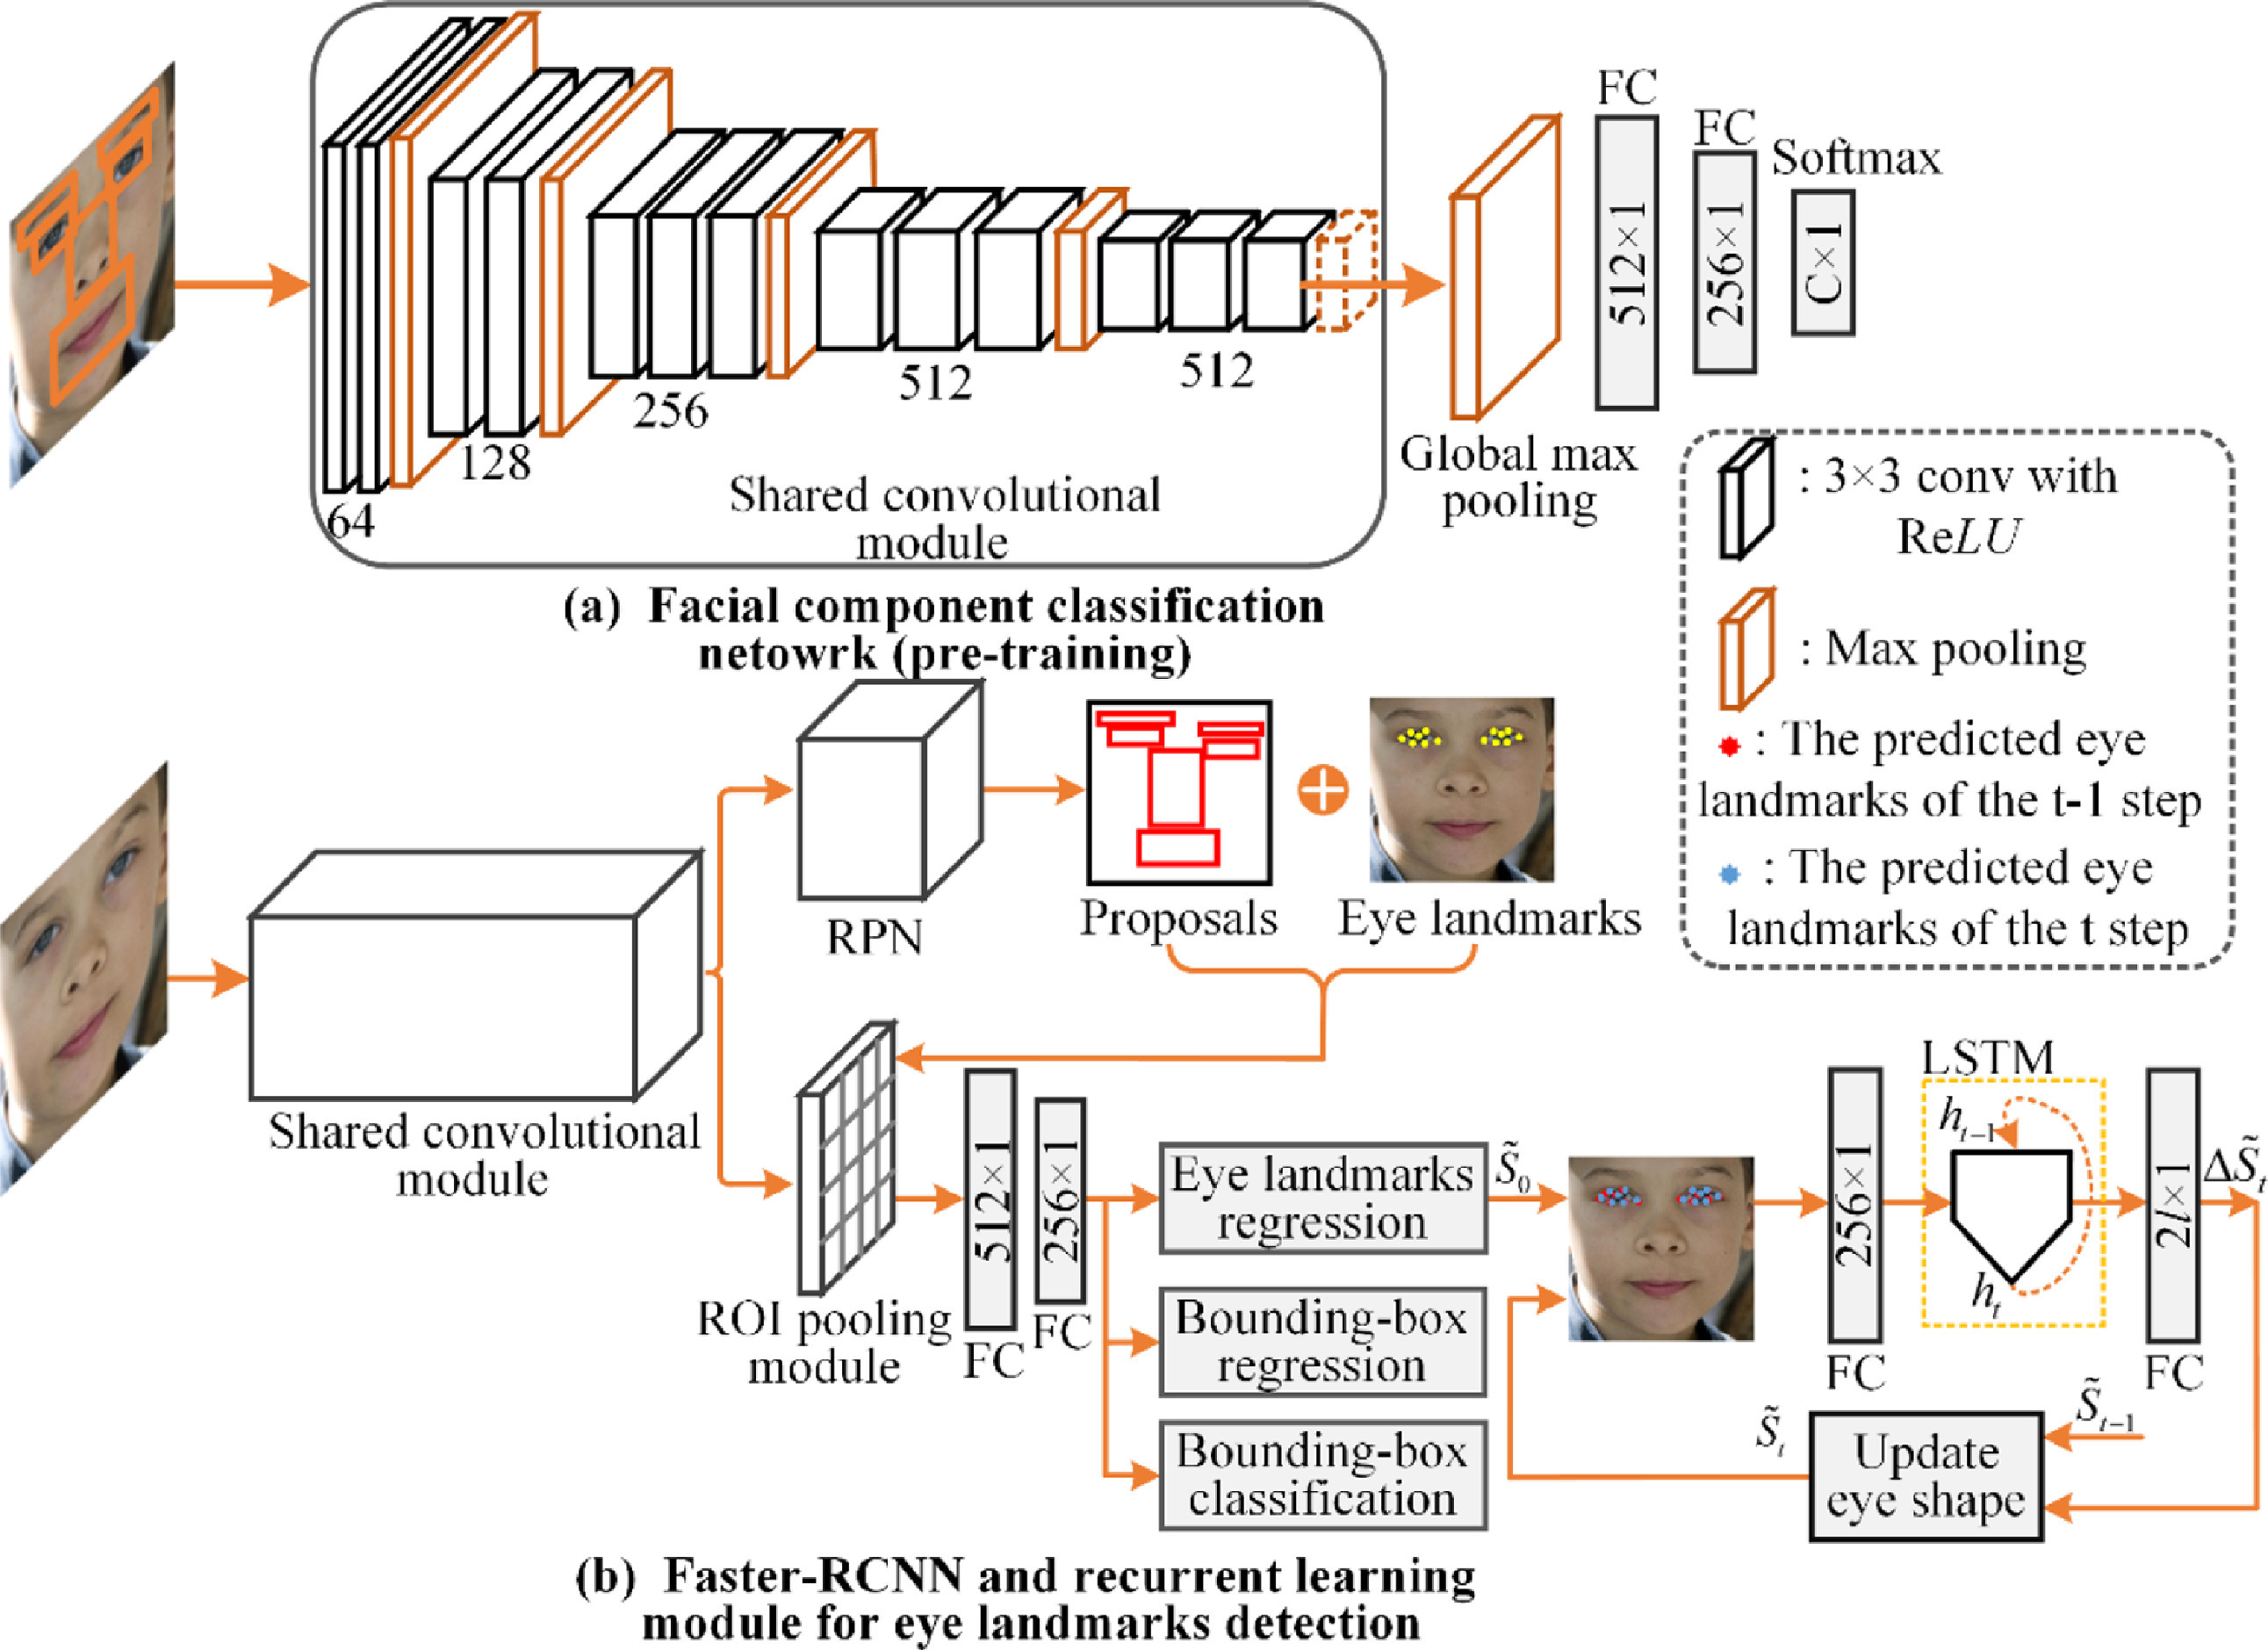
\includegraphics[width=0.75\linewidth]{dissertation//figures/wseld.jpg}
    \caption{Network diagram of Weakly Supervised Eye Landmarks Detection\cite{huang2020eye}}
    \label{fig:wseld}
\end{figure}

Whilst the original paper gave clear implementations, their code was difficult to replicate. No code was supplied with the paper so all code had to be generated from scratch. The most confusing aspect of the model was generating landmarks from an RPN. As the name suggests, RPNs are only able to generate regions, as such it would seem to be impossible to generate landmarks. A similar paper was able to produce results on multiple facial regions\cite{tang2018facial} but, again, no code was provided. In this implementation it was assumed a dense layer with the number of outputs equal to the number of landmarks was incorporated into the output of the RPN. Furthermore, this was the author's first time coding a substantial learning framework in TensorFlow. There is no pre-built RPN module so one needs to be created from scratch, a number of open source implementations exist\cite{hxuaj2021tensorflow2}\cite{kewar2021region} but these do not generate landmarks. It was attempted to create a custom R-CNN but there was a seeming constant stream of bugs. The bugs, along with there being no way to confirm whether the method of adding landmarks to RPN was successful resulted in development of WSELD being halted in favour of a new facial landmarking network.

\subsubsection{Pre-implemented Models}

% \begin{itemize}
%     \item Re-use oriented design
%     \item papers with code
%     \item Used best models which had pre-existing implementations (one for fast, one more accurate)
%     \item couldve optimised for 6 landmarks but didnt want to mess with model architectures that were known working (batch size probably meant nothing would change anyway)
% \end{itemize}

To avoid a repetition of the WSELD implementation, it was decided to switch to a re-use oriented methodology for facial landmarking. In order for a model to be considered, it must have an open source implementation available. PapersWithCode\footnote{\url{https://paperswithcode.com}} is an aggregation site which ranks models on popular machine learning problems and links to known codebases where possible. 

The facial landmark detection is a common problem in machine learning. The vast majority of available training datasets (Section \ref{sec:face-datasets}) contain the six points required for EAR calculation and as such any model that can be trained on these datasets can be used for eye landmarking. In theory, it is possible to optimise the networks for solely eye landmark detection, however this will not be optimised due to the potential that had to disrupt a network that is known to be working.

\subsubsection{High-Resolution Network}

% \begin{itemize}
%     \item modular sequences
%     \item keeps high resolution layers in context at all times
%     \item generic network but with a specific implementation for eye landmarking
%     \item Heatmap per landmark
% \end{itemize}

The most implemented facial landmark detector on PapersWithCode is High-Resolution Network (HRNet)\cite{sun2019high}. HRNet is actually a proposal for a novel architecture of CNNs that has applications in many fields and one of those fields is facial landmarking.

HRNet's novel contribution is parallel fusion blocks 

\subsubsection{PFLD}

\begin{itemize}
    \item speedy boi
    \item uses mobilenet-techniques to reduce the size and increase the speed
    \item still accurate tho
    \item secret sauce is custom loss function
\end{itemize}

\subsubsection{Facial Landmark Datasets}
\label{sec:face-datasets}

\begin{itemize}
    \item 68 landmarks (upsampling and downsampling where necessary)
    \item list all of them and give brief overview
    \item didnt use aflw due to inaccurate landmarks or not enough landmarks
    \item reflected to double size
\end{itemize}

\subsubsection{Final model choice}

Yunet + PFLD, then MTCNN and HRNET as backup (hope ear analysis can filter out idiosyncrasies of the model as will be consistent across real and fake)

\subsection{EAR Analysis}

\begin{itemize}
    \item Can be abstracted to a univariate time series
    \item Well researched
    \item Classical methods exists (pyts library)
    \item explain each one and give simple summary (1 paragraph)
    \item As do deep learning frameworks (the other papers)
    \item model diagrams for each one (maybe give a rough explenation as to the aims each one is doing?)
\end{itemize}

\section{Adversarial Noise}

\begin{itemize}
    \item foolbox library (Targeted FGSM using the other thing)
    \item chosen over cleverhans as cleverhans had meh documentation
    \item cw-l2 attack too slow (3hrs per video)
    \item fakeretouch has no open-source implementation, timings were too slow, estimated would also take a while
\end{itemize}

\section{Final Code}

\begin{itemize}
    \item One codebase to do full training, splitting and evaluation
    \item just give overall flow diagram?
    \item {\huge models only trained on non-noisy images}
    \item checkpointing where possible
    \item run on either dcs compute clusters or avon
    \item final speeds + hardware
\end{itemize}